\chapter{實驗與執行結果}
%\label{c:intro}
本章節討論網頁與分析的結果與輸出數據
\section{網頁平台數據結果}
\subsubsection{顯示頁面}
在網頁的平台只有觀察使用者打字與紀錄時間並畫圖顯示。(圖4.1)為網頁偵測的頁面,中間的空白處就是給使用者打字的地方,並且在進行打字同時計算字數回傳,進而畫出時間字數的折線圖。
	\begin{figure}[H] 
	\centering 
	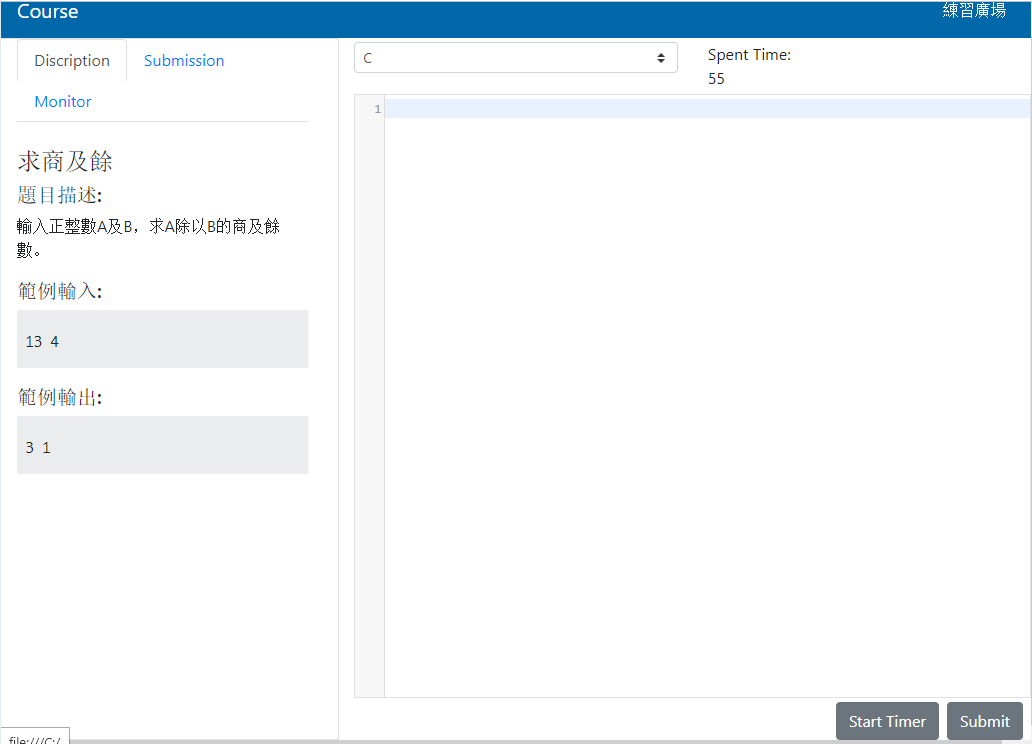
\includegraphics[width=0.7\textwidth]{web_part.png} 
	\caption{網頁顯示頁面} 
	\label{Fig.4.1} 
	\end{figure}
\subsubsection{網頁的圖形輸出}
首先先觀察monitor檔所抓到的數據與圖形的顯示。
因本研究是基於討論學生在做題目的分析,於是我找了一些文字試打並擷取monitor檔的圖形畫面結果:
\begin{enumerate}[1.]
	\item 簡短程式碼(圖4.2)\\
	左邊部分為html的網頁使用者介面,右邊為monitor檔所呈現的的圖形數據,並且圖上可以看出在打字時若遇到打錯的地方,所使用backspace倒退鍵的情況也變多了,所以圖上呈現才會有更多的彎曲;上升一點下降一點就是使用者在改錯的地方。
	\begin{figure}[H] 
		\centering 
		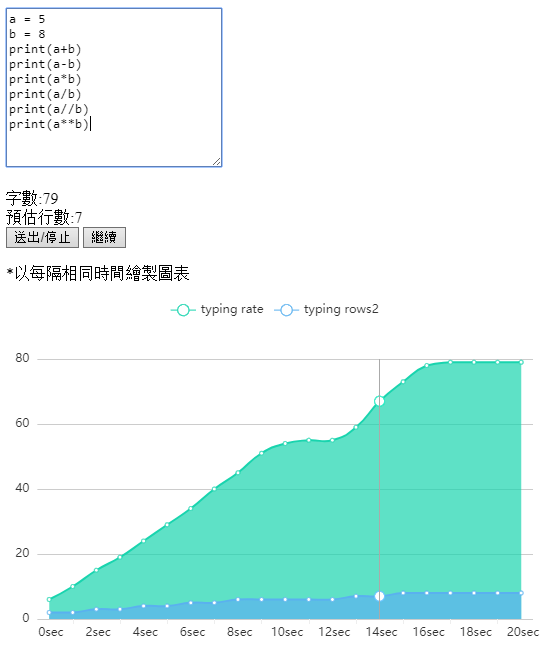
\includegraphics[width=0.7\textwidth]{4_2.png} 
		\caption{簡短程式碼輸出} 
		\label{Fig.4.2} 
	\end{figure}
	\item console的訊息(圖4.3)\\
	把上面打到一半的程式繼續往下打,並且把console打開觀察,可以看到每當網頁介面的數據有所變化時,monitor檔便會知曉每次增加或減少的變動,進而把數據顯示在圖形與網頁上。右邊console部分更可以看出什麼時間的時候程式碼進行到哪一部分。在此設定為3秒鐘取一次,能在console清楚的看到,之所以不需要太密集取值是因為適量的調控數據使數據不要太多或過於繁雜,若是一次取太多值,則需要更多的空間存取,如此之後的存取與分析會變得更加複雜。因此在此處只設定3秒鐘取一次。
	\begin{figure}[H] 
		\centering 
		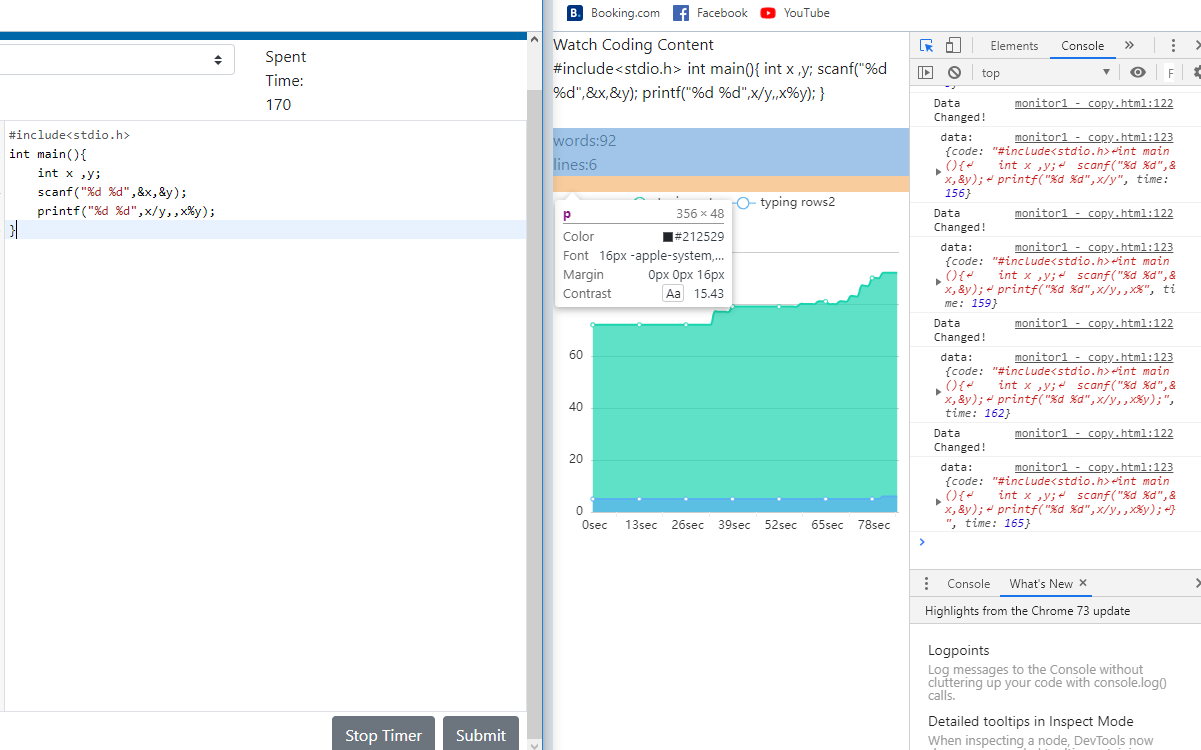
\includegraphics[width=0.7\textwidth]{4_3.png} 
		\caption{console的訊息} 
		\label{Fig.4.3} 
	\end{figure}
	\item 複製貼上(圖4.4)\\
	若是使用者貼上大量文字的話,圖形變化會成階梯狀因數據變化的幅度比自行打字大很多,此為模擬若是使用者頻繁的貼上。因此如使用者使用了貼上鍵,此頁面是能夠偵測到的。
	\begin{figure}[H] 
		\centering 
		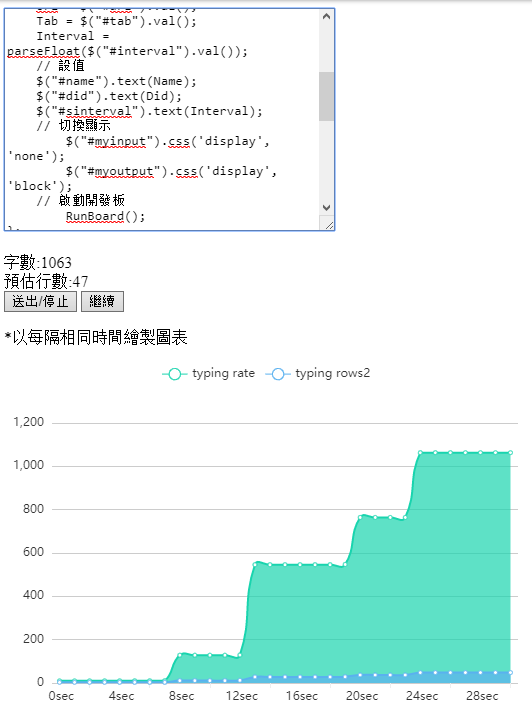
\includegraphics[width=0.7\textwidth]{4_4.png} 
		\caption{複製貼上輸出} 
		\label{Fig.4.4} 
	\end{figure}
\end{enumerate}
\subsubsection{網頁的影片輸出}
除了在monitor檔或是monitor檔裡的console中可以觀察使用者在打字的時候的動作外,把這些數據綜合起來則可以統整成一個影片並且輸出。以下稱此功能的檔案為makevideo檔。\\
\begin{itemize}
	\item makevideo檔的運作:\\
	打開makevideo檔會是一個空白的框(圖4.5)
		\begin{figure}[H] 
		\centering 
		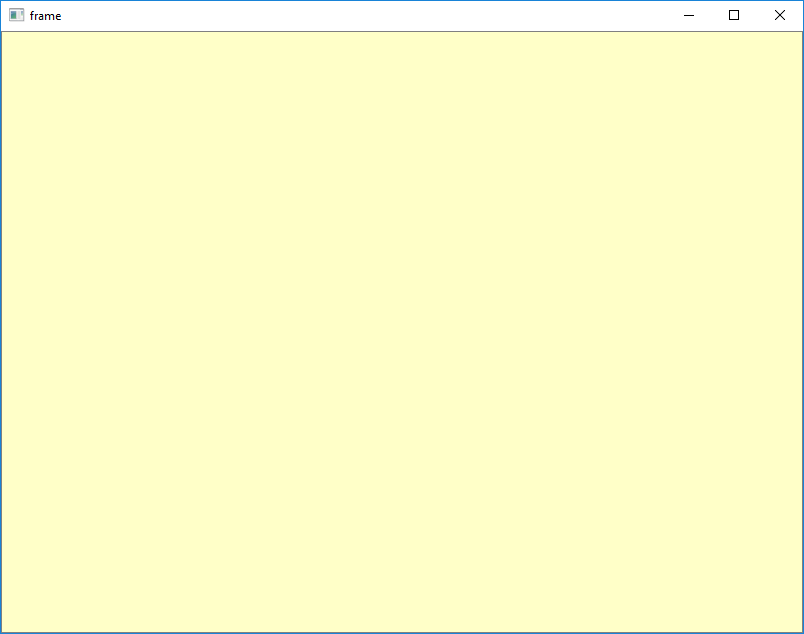
\includegraphics[width=0.7\textwidth]{video_space.png} 
		\caption{makevideo檔初始} 
		\label{Fig.4.4.1} 
		\end{figure}
	並且當使用者在打字的介面開始打字時,此框便也會開始動作。前面也提到此數據也是經由firebase傳送的數據進行更新;也就是當使用者在一邊打字時,此makevideo檔也會跟著觀察更新使用者所打的字在框框上。\\(圖4.6)
	\begin{figure}[H] 
		\centering 
		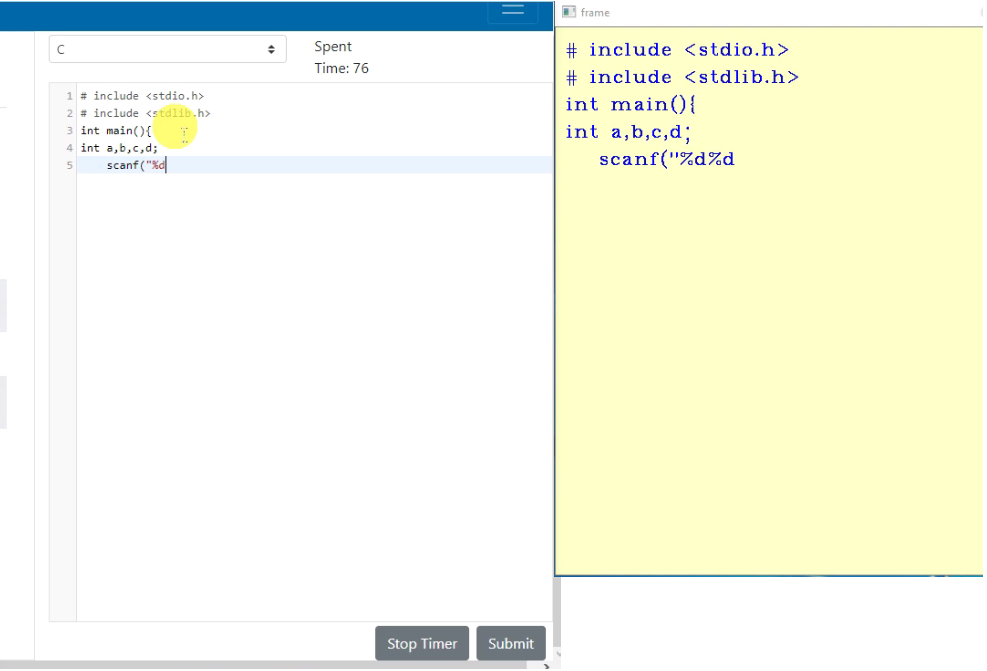
\includegraphics[width=0.7\textwidth]{frame.png} 
		\caption{makevideo檔與網頁介面} 
		\label{Fig.4.4.2} 
	\end{figure}

	在結束擷取之後,便會把這些被觀察的使用者動作輸出成影片並且存取為一個AVI影片檔。
	
	\item 影片動作與實際動作:\\
	makevideo檔輸出後的AVI所發生的動作就跟執行makevideo檔所呈現的框裡的動作一樣。在此想把輸出的AVI影片檔與真正打字的影片檔做比較,於是在打字的時候一邊錄了螢幕錄影。\\
	(圖4.7)為螢幕錄影的影片與makeevideo所產生的影片比較。
		\begin{figure}[H] 
		\centering 
		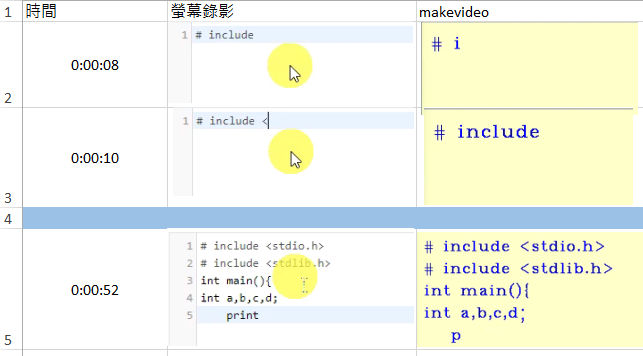
\includegraphics[width=0.7\textwidth]{diff.png}
		\caption{螢幕錄影與makevideo比較} 
		\label{Fig.4.4.3} 
		\end{figure}
	可以看出影片的動作會慢於實際的打字速度,因為在取值時有設定固定的秒數,因此若是使用者不間斷的打字必然不能完整呈現,所以makevideo檔所產生的輸出影片與實際上螢幕錄影影片是延遲的。\\
	但是此種方法確實可以很好的模擬使用者在打字時後的種種動作。
	\item python檔:\\
	在前面架構與規劃有提到,不只是可以呈現網頁上的數據圖形與影片,也多撰寫一個python程式同樣經由firebase把使用者的打字狀況抓下來。抓下來的目的是因為之所使用的分析程式大量使用python。(圖4.8)
	\begin{figure}[H] 
		\centering 
		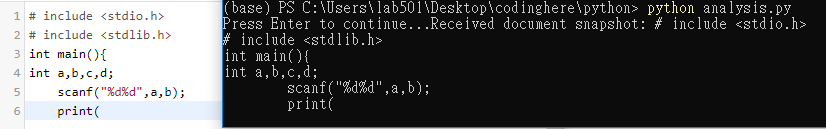
\includegraphics[width=0.7\textwidth]{anysis.png}
		\caption{python抓下的文字} 
		\label{Fig.4.4.4} 
	\end{figure}
\end{itemize}

\section{python的討論分析}
因本研究所寫的python程式碼可以指定實驗數據的數量進進行製作與分析,在此便指定10組與30組結果。
\subsubsection{個別的圖形與數據}
每一組數據便會產生(圖4.9)的一組圖形,在此便不把全部圖形列出,以下只列每次產生的數據最基本的折線圖,共10組。(圖4.10)
	\begin{figure}[H] 
	\centering 
	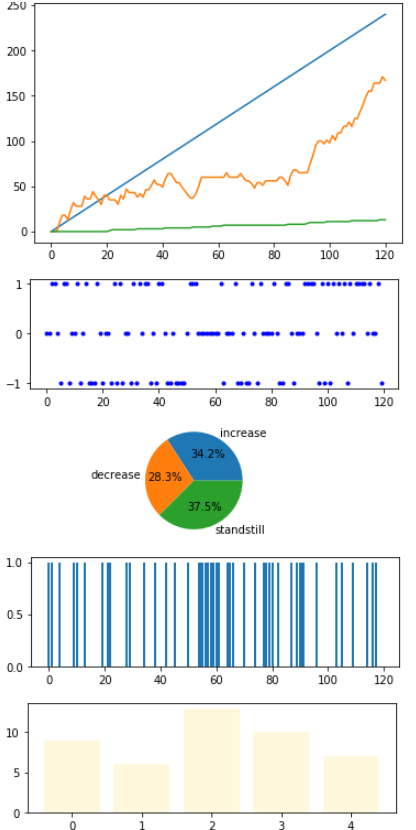
\includegraphics[width=0.7\textwidth]{4_5.png} 
	\caption{圖形組} 
	\label{Fig.4.5} 
	\end{figure}
	\begin{figure}[H] 
	\centering 
	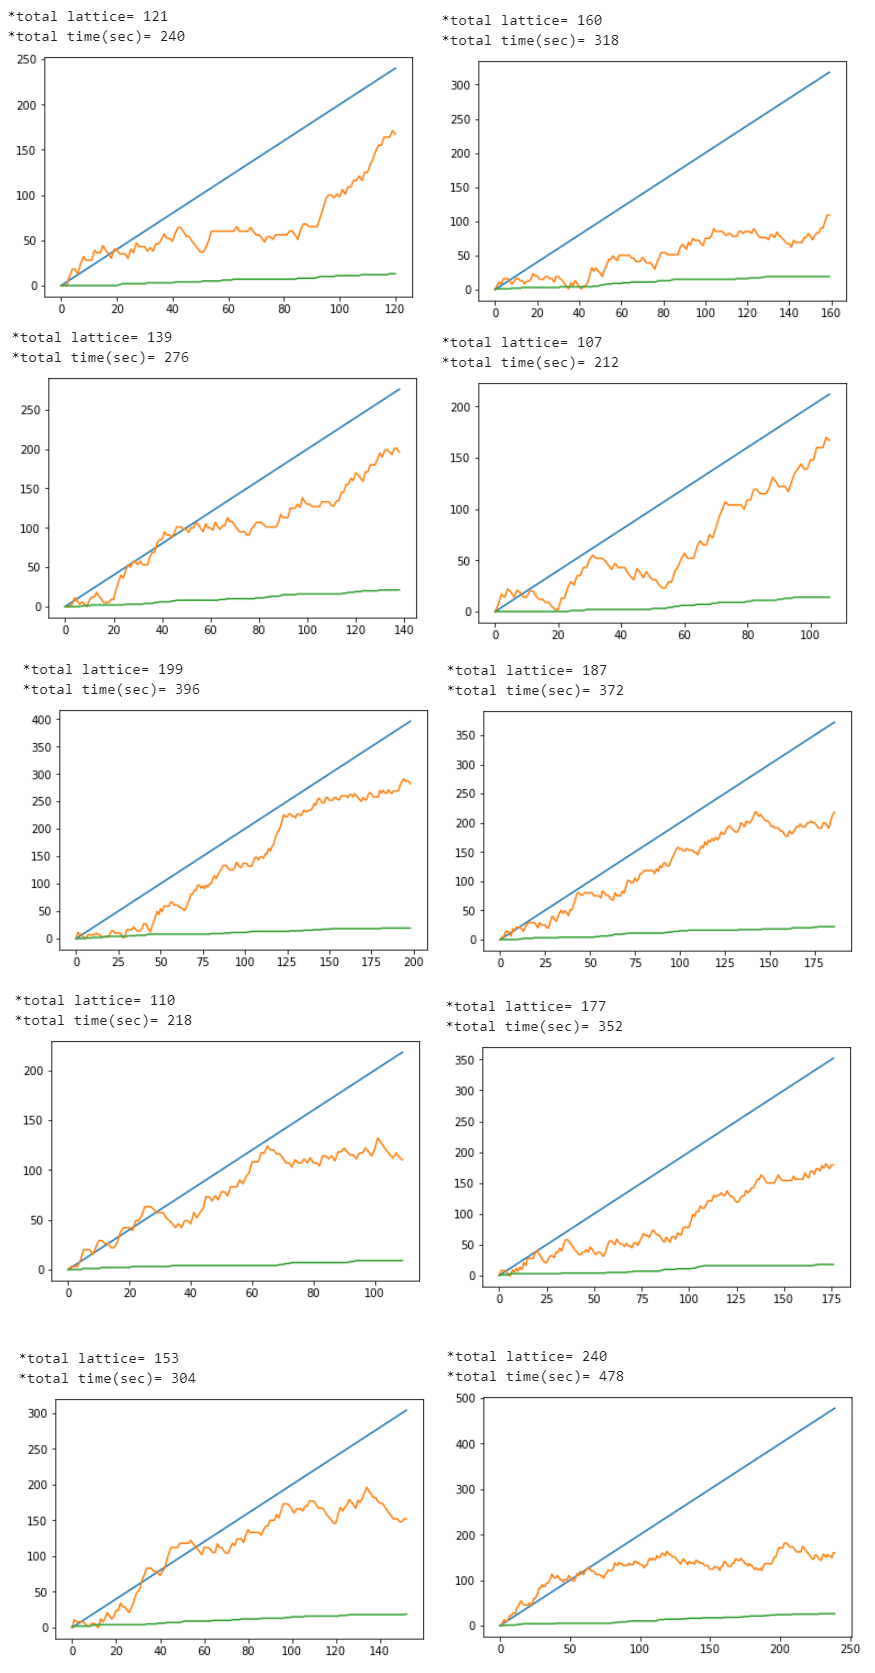
\includegraphics[width=0.7\textwidth]{4_6.png} 
	\caption{10組折線圖} 
	\label{Fig.4.6} 
	\end{figure}
\subsubsection{統整的表格數據}
把全部的數據統整起來製程表格,表格也是使用python在colab可以輸出顯示結果。\\
1. 10組結果(圖4.11)
	\begin{figure}[H] 
	\centering 
	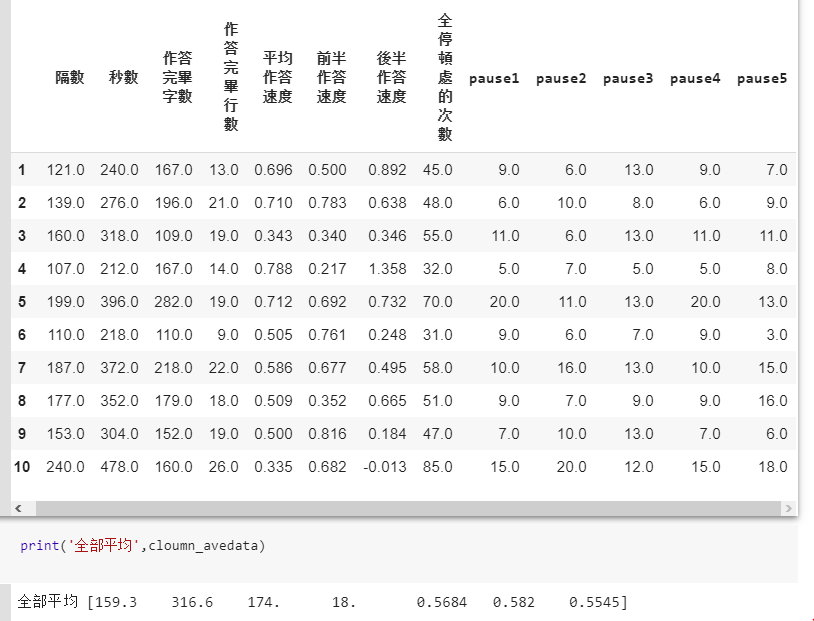
\includegraphics[width=0.7\textwidth]{4_7.png} 
	\caption{10組結果表格圖} 
	\label{Fig.4.7} 
	\end{figure}
\newpage
2. 30組結果,因資料較龐大所以使用表格顯示(表4.1))\\
\begin{table}[]
	\label{table1}
	\begin{tabular}{lllllllll}
		& 隔數  & 秒數  & 作答完畢字數 & 作答完畢行數 & 平均作答速度 & 前半作答速度 & 後半作答速度 & 全停頓處的次數 \\
		1  & 115 & 228 & 193    & 19     & 0.846  & 0.833  & 0.86   & 39      \\
		2  & 190 & 378 & 343    & 14     & 0.907  & 0.984  & 0.831  & 72      \\
		3  & 212 & 422 & 230    & 26     & 0.545  & 0.417  & 0.673  & 69      \\
		4  & 149 & 296 & 204    & 12     & 0.689  & 0.716  & 0.662  & 52      \\
		5  & 172 & 342 & 246    & 17     & 0.719  & 0.374  & 1.064  & 53      \\
		6  & 135 & 268 & 94     & 15     & 0.351  & 0.425  & 0.276  & 46      \\
		7  & 219 & 436 & 299    & 26     & 0.686  & 0.583  & 0.789  & 67      \\
		8  & 133 & 264 & 189    & 19     & 0.716  & 0.803  & 0.629  & 51      \\
		9  & 111 & 220 & 171    & 11     & 0.777  & 1.509  & 0.045  & 31      \\
		10 & 127 & 252 & 80     & 15     & 0.317  & 0.516  & 0.119  & 47      \\
		11 & 140 & 278 & 242    & 19     & 0.871  & 0.964  & 0.777  & 51      \\
		12 & 241 & 480 & 288    & 26     & 0.6    & 0.354  & 0.846  & 77      \\
		13 & 222 & 442 & 371    & 25     & 0.839  & 1.009  & 0.67   & 70      \\
		14 & 220 & 438 & 288    & 28     & 0.658  & 0.749  & 0.566  & 71      \\
		15 & 247 & 492 & 218    & 28     & 0.443  & 0.472  & 0.415  & 84      \\
		16 & 158 & 314 & 176    & 18     & 0.561  & 0.924  & 0.197  & 52      \\
		17 & 162 & 322 & 136    & 17     & 0.422  & 0.472  & 0.373  & 61      \\
		18 & 227 & 452 & 267    & 29     & 0.591  & 0.633  & 0.549  & 81      \\
		19 & 199 & 396 & 139    & 19     & 0.351  & 0.641  & 0.061  & 75      \\
		20 & 240 & 478 & 209    & 32     & 0.437  & 0.552  & 0.322  & 75      \\
		21 & 202 & 402 & 178    & 25     & 0.443  & 0.597  & 0.289  & 61      \\
		22 & 189 & 376 & 349    & 22     & 0.928  & 0.793  & 1.064  & 53      \\
		23 & 203 & 404 & 161    & 26     & 0.399  & 0.302  & 0.495  & 65      \\
		24 & 146 & 290 & 197    & 8      & 0.679  & 1.186  & 0.172  & 48      \\
		25 & 195 & 388 & 185    & 17     & 0.477  & 0.629  & 0.325  & 70      \\
		26 & 93  & 184 & 61     & 10     & 0.332  & 0.946  & -0.283 & 25      \\
		27 & 98  & 194 & 60     & 2      & 0.309  & 0.33   & 0.289  & 28      \\
		28 & 93  & 184 & 132    & 8      & 0.717  & 0.772  & 0.663  & 33      \\
		29 & 204 & 406 & 225    & 18     & 0.554  & 0.951  & 0.158  & 65      \\
		30 & 120 & 238 & 91     & 16     & 0.382  & 0      & 0.765  & 52     
	\end{tabular}
\caption{30組數據}
\end{table}
\newpage
\section{結果討論}
\subsection{html網頁偵測部份}
\begin{itemize}
	\item 本研究藉由網頁前端及時偵測使用者的打字情況,並且計算其字數與花費時間。不同於其餘答題系統需要繳交後才知曉使用者的答題狀況,此方法因為其實時偵測的特性,使用者的答題習慣也可以藉由字數與時間看出端倪。
	\item 在網頁上只擷取了字數、行數與時間,如可以增加更多的鍵盤偵測將會使系統更加完善,此處為能多加以改良完善的地方。
	\item 在影片輸出部分,本研究比較了經由網頁數據形成的影片與實際使用螢幕錄影的效果,雖輸出的影片不及真正的錄影資訊來的完整與細緻,但輸出的影片能明確抓取使用者在網頁進行的改動。
\end{itemize}
\subsection{python分析部分討論}
\begin{itemize}
	\item 進行分析的部分最大的難處就是缺少實際數據,因此在本文中使用程式去模擬實際的數據。但是因在此使用大量的radom函數與諸多限制,如為了使程式撰寫方便設的上下界線使數據密集化等。模擬的數據理所當然地不及實際數據來的真實與客觀。
	\item 再討論數據停頓的密集程度的地方(圖3.16),我所選用的方法是把整體數據分成五個等分並寫計算每一等分的停頓次數;而此部分也是不夠嚴謹的,因可能密集的地方會被分組計算而分割,所以分區計算的方法並不能表示絕對的疏密程度。
\end{itemize}